% Created 2024-01-09 Tue 09:14
% Intended LaTeX compiler: xelatex
\documentclass[10pt,twoside,landscape]{article}
\usepackage{graphicx}
\usepackage{longtable}
\usepackage{wrapfig}
\usepackage{rotating}
\usepackage[normalem]{ulem}
\usepackage{amsmath}
\usepackage{amssymb}
\usepackage{capt-of}
\usepackage{hyperref}
\usepackage{subcaption}
\usepackage[newfloat]{minted}
\usepackage{color}
\usepackage{listings}
\usepackage[top=2cm,bottom=2cm,right=2cm,left=2cm,landscape]{geometry}
\usepackage{multicol}
\usepackage{enumitem}
\usepackage{fancyhdr}
\usepackage{caption}
\usepackage{algorithm}
\usepackage{algpseudocode}
\usepackage{float}
\setlist[description]{itemsep=-1pt,leftmargin=2mm,topsep=0pt}
\setlist[itemize]{itemsep=-1pt,topsep=0pt}
\setlist{noitemsep}
\setlength{\parindent}{0pt}
\setlength{\columnseprule}{0.2pt}
\definecolor{mygreen}{rgb}{0,0.6,0}
\definecolor{mygray}{rgb}{0.5,0.5,0.5}
\definecolor{mymauve}{rgb}{0.58,0,0.82}
\lstset{ backgroundcolor=\color{white}, basicstyle=\footnotesize, breaklines=true, captionpos=b, commentstyle=\color{mygreen}, escapeinside={\%*}{*)},keywordstyle=\color{blue}, stringstyle=\color{mymauve},}
\author{Olivier Lischer}
\date{\today}
\title{WE3 Exam Summary}
\hypersetup{
 pdfauthor={Olivier Lischer},
 pdftitle={WE3 Exam Summary},
 pdfkeywords={},
 pdfsubject={},
 pdfcreator={Emacs 29.1 (Org mode 9.7-pre)}, 
 pdflang={English}}
\begin{document}

\pagestyle{fancy}
\fancyhf{}
\fancyhead[R]{WE3-HS23}
\fancyhead[L]{Exam Summary}
\fancyfoot[CE,CO]{\leftmark}
\fancyfoot[R]{\thepage}
\fancyfoot[L]{Olivier Lischer}

\begin{multicols}{4}
\section{SPA}
\label{sec:org261e7bb}
\subparagraph{What are the benefits of a browser based application?} \
\label{sec:org1214653}
A browser based application (web application) has various benefits:
\begin{itemize}
\item You can work from anywhere at anytime
\item It is platform independent (even mobile)
\item No software update nor installation => easy maintenance
\item Software can provided as a Services (SaaS)
\item Can be cross-compiled to different ecosystems
\end{itemize}
\subparagraph{What are the liabilities of a browser based application?} \
\label{sec:org80b24fd}
Browser based applications do not have only benefits but also downsides, such as:
\begin{itemize}
\item no data sovereignty
\item limited / restricted hardware access (no OS access, may be less efficient)
\item Search Engine Optimization (SE must execute JS)
\item More complex deployment strategies
\item Overhead
\end{itemize}
\subparagraph{What are characteristics of an SPA?} \
\label{sec:orgef02694}
An SPA has the following properties:
\begin{itemize}
\item Plan HTML5 / CSS and JavaScript
\item no page reloads
\item Working Back-Button
\item Bookmarkable Links
\item Provides (limited) offline functionality
\item Uses (\href{../../../roam/20230108172748-what_is_rest.org}{REST})-API services for data access
\end{itemize}
\subparagraph{When would you prefer an SPA to a classic web application from the customer's point of view?} \
\label{sec:org0945583}
As soon as a desktop (native) app with a similar user experience is required.
\subparagraph{What do you see as the technical benefits of an SPA?} \
\label{sec:org420985f}
The server application is separated from the display by a structured interface (e.g. REST / ODATA / WSDL). This opens up various advantages:
\begin{itemize}
\item Seperation of Concerns
\item Better maintainability of the client code
\item Division into different teams / competence centers
\end{itemize}
\subparagraph{What does a typical layering in an SPA look like?} \
\label{sec:org8009e4b}
The Views are connected using a routing in the browser.
The Business Logic provides data over servies and only the data layer will communicate directly with the server.

{
\begin{center}
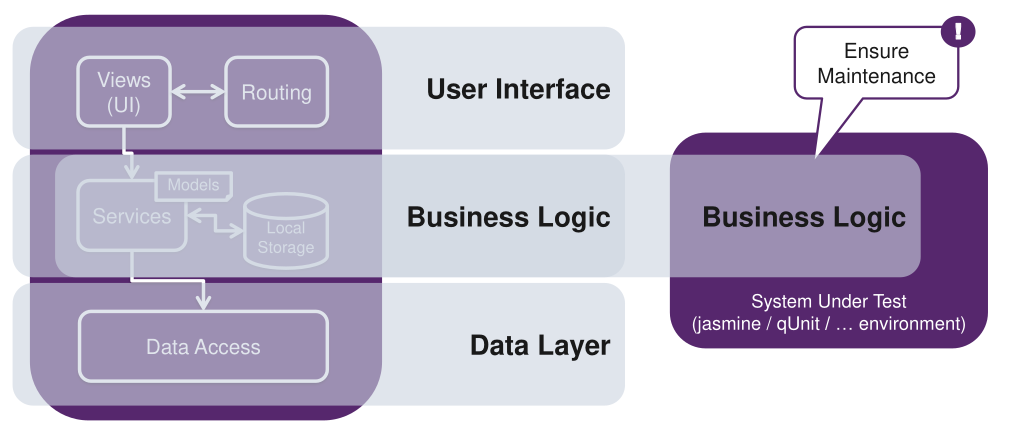
\includegraphics[width=.9\linewidth]{img/spa_layering.png}
\end{center}
\captionof{figure}{Layering in SPA}\label{fig:layering-in-spa}
}
\subparagraph{Why do we use bundling in an SPA?} \
\label{sec:orge416d5d}
An SPA may consist of many single JS files, which may or may not dependt on each other.
To include them manually in your HTML is error pronce and tedious.

With bundling we achive the following things:
\begin{itemize}
\item All JS code must be delivered to the client over potentially metered/slow networks
\item Bundling and minifying the source leads to smaller SPA footprint (e.g. using \href{../../../roam/20231228113108-what_is_tree_shaking.org}{Tree Shaking})
\item Bundling leads to a reliable dependency management
\item Usage of pre and post processors during bundling
\end{itemize}


The initial footprint caused by bundling can be reduced by loading dependent modules on-demand.
\section{React}
\label{sec:orgec34e72}
\subparagraph{How do you make props available for all child components?} \
\label{sec:orgccef24e}
However, you should only use contexts for read-only variables and limit the number of different contexts.

\begin{itemize}
\item \texttt{React.createContext()}
\item \texttt{<TContext.Provider value=\{value\}></TContext.Provider>}
\item \texttt{useContext}
\end{itemize}
\subparagraph{How does Redux work?} \
\label{sec:org20b9d60}
The state in Redux is represented as trees of objects.
The tree is immutable.
When you change something in the tree, a new tree will be created (\href{../../../roam/20220616080932-functional_programming.org}{Functional Programming}).

A state action is communicated using a \emph{Redux Action}.
A \emph{Reducer} takes the action and the current state an applies the action on the state to generate a new state.

{
\begin{center}
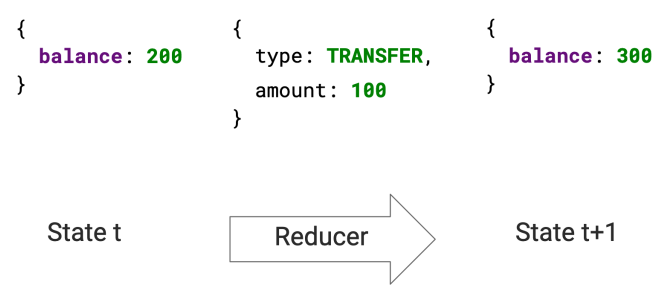
\includegraphics[width=.9\linewidth]{img/redux_action_reducer.png}
\end{center}
\captionof{figure}{Action Reducer State change}\label{fig:action-reducer-state-change}
}
\section{Angular}
\label{sec:orge90f293}
\subparagraph{Angular Architectural Parts} \
\label{sec:org20f8710}
ngModules, directives, components, templates, metadata, services
\subparagraph{Angular Module Declaration} \
\label{sec:orgdf37130}
\begin{itemize}
\item declarations: belongs to this module
\item exports: Subset of declarations
\item imports: imported into this module
\item providers: Creators of services, contributes to the global DI container
\item bootstrap: Main application view (only in root module)
\end{itemize}
\subparagraph{Binding Syntax} \
\label{sec:org075ed2e}
{
\begin{minted}[]{html}
<!-- Two Way Binding -->
<input
  type="text"
  [(ngModel)]="counter.team">

<!-- One Way (View to Model) -->
<button
  (click)="counter.eventHandler($event)">

<!-- One Way (Model to View) -->
<p>{{counter.team}}</p>
\end{minted}
\captionof{listing}{Bindings variants in Angular}\label{lst:bindings-variants-in-angular}
}
\subparagraph{Directives} \
\label{sec:orgaf39057}
Declared as a TypeScript class with an \texttt{@Directive()} function decorator.
\textbf{Structural} directive: modifies structure of DOM (\texttt{*ngIf} / \texttt{*ngFor}), \textbf{Attribute} directive: alters appereance / behavior of an existing element (\texttt{[ngStyle]} / \texttt{[ngClass]})
\subparagraph{Services} \
\label{sec:org385358a}
The \texttt{@Injectable} decorater is used to register the service in the DI container.
\texttt{@Injectable(\{ providedIn: 'root' \})export class CounterService \{\}}
\subparagraph{Forms} \
\label{sec:org04e7727}

{
\begin{minted}[]{html}
<form #f="ngForm"
  (ngSubmit)="doLogin(f)">
</form>
\end{minted}
\captionof{listing}{Angular Form Markup}\label{lst:angular-form-markup}
}

{
\begin{minted}[]{typescript}
@Component({})
export class SampleComponent {
  public doLogin(f?: NgForm) {
    if (f?.form.valid) {}
    return false;
  }
}
\end{minted}
\captionof{listing}{Angular Form Logic}\label{lst:angular-form-logic}
}
\subparagraph{Routing} \
\label{sec:orgb830c24}
\texttt{.forRoot()}: declare routes on root level, \texttt{.forChild()} declaring sub-routings
\subparagraph{Module Type / Example Architecture} \
\label{sec:org38d2913}
Root / App Module, Feature Modules, Shared Module, Core Module
\subparagraph{RxJS - Observable Types} \
\label{sec:org2a9da78}
Hot Observables, Cold Observables (triggerd on subscription)
\subparagraph{Pipes} \
\label{sec:org20ff179}
Pure Pipes (change to the input expression), Impure Pipes (executed on every change detection cycle)
\section{ASP.NET}
\label{sec:orgca46951}
\subparagraph{PWA} \
\label{sec:orgbd677ad}
PWA use modern web APIs along with traditional progressive enhancement strategy (fells like native app)
\subparagraph{For what is Firbase used?} \
\label{sec:org692b7ac}
To develop a PWA we used the following features from Firebase:
\begin{itemize}
\item Cloud Firestore / Realtime (DB)
\item Cloud Functions (Serverless Functions)
\item Authentication
\item Hosting / Cloud Storage
\end{itemize}
\subparagraph{Front Controller} \
\label{sec:org8f6da09}
The Front Controller is the Entry Point and executes logging and routing (actions that are required for all incoming requiest).
After that, the front controller forwards the request the the responsible controller.
\subparagraph{Middleware} \
\label{sec:orgc3f0823}
Middleware is a "function block" and has a certain task.
When a middleware has finished its task it will call the next following middleware or finishes the request.
\begin{itemize}
\item \texttt{app.Use()}: non terminating
\item \texttt{app.Map()}: mapping
\item \texttt{app.Run()}: terminating
\item \texttt{app.UseMiddleware<>()}: register class middleware
\end{itemize}

Context contains all information for the request as well for the response.
\subparagraph{Dependency Injection - Lifetime} \
\label{sec:orgc36ff79}
Register services with different lifetimes:
\begin{itemize}
\item Transient, are created every time when used
\item Scoped, are created once for every request (used most often)
\item Singelton, it's just a singelton (only for Readonly, configs, options)
\end{itemize}


Register a transient service: \texttt{builder.Services.AddTransient<>()}


\textbf{Captive dependency}
The term "captive dependency" refers to the misconfiguration of service lifetimes, where a longer-lived service holds a shorter-lived service captive.
\begin{itemize}
\item Transient requires Singelton -> OK
\item Singelton requires Transient -> Not OK
\begin{itemize}
\item When the singleton is used a 2nd time (e.g. parallel) it uses the same reference to the transient service.
\item Transient services are normally \textbf{NOT} thread-safe and an error can occuer when used in a not thread safe context
\end{itemize}
\end{itemize}
\subparagraph{Web Assembly File Type} \
\label{sec:org9a206ff}
\begin{itemize}
\item *.WASM (WebAssembly)
\begin{itemize}
\item Compiled Web Assembly
\item Can be transformed back to WAT
\end{itemize}

\item *.WAT
\begin{itemize}
\item Text Based Web Assembly
\item Can be compiled to WASM
\end{itemize}

\item Web Assembly
\begin{itemize}
\item Is a stack machine (similar to the JVM)
\item \href{../../../roam/20221230171752-what_is_a_evaluation_stack.org}{Evaluation Stack}
\end{itemize}
\end{itemize}
\subparagraph{Key Concepts} \
\label{sec:orgf0b797d}
\begin{itemize}
\item Module
\begin{itemize}
\item Represents a WebAssembly binary that has been compiled by the browser into executable machine code
\item Stateless
\item Import / Export
\end{itemize}
\item Memory
\begin{itemize}
\item shared memory section between JS and web assembly
\end{itemize}
\item Table
\begin{itemize}
\item A resizable typed array of references (e.g. to functions) that could not otherwise be stored as raw bytes in Memory (for safety and portability reasons).
\end{itemize}
\item Instance
\begin{itemize}
\item A Module paired with all the state it uses at runtime including a Memory, Table, and set of imported values.
\end{itemize}
\end{itemize}


\end{multicols}
\end{document}
